%%%%%%%%%%%%%%%%%%%%%%%%%%%%%%%%%%%%%%%%%
% Beamer Presentation
% LaTeX Template
% Version 1.0 (10/11/12)
%
% This template has been downloaded from:
% http://www.LaTeXTemplates.com
%
% License:
% CC BY-NC-SA 3.0 (http://creativecommons.org/licenses/by-nc-sa/3.0/)
%
%%%%%%%%%%%%%%%%%%%%%%%%%%%%%%%%%%%%%%%%%

%----------------------------------------------------------------------------------------
%	PACKAGES AND THEMES
%----------------------------------------------------------------------------------------

\documentclass{beamer}

\mode<presentation> {

% The Beamer class comes with a number of default slide themes
% which change the colors and layouts of slides. Below this is a list
% of all the themes, uncomment each in turn to see what they look like.

%\usetheme{default}
%\usetheme{AnnArbor}
%\usetheme{Antibes}
%\usetheme{Bergen}
%\usetheme{Berkeley}
%\usetheme{Berlin}
%\usetheme{Boadilla}
%\usetheme{CambridgeUS}
%\usetheme{Copenhagen}
%\usetheme{Darmstadt}
%\usetheme{Dresden}
%\usetheme{Frankfurt}
%\usetheme{Goettingen}
%\usetheme{Hannover}
%\usetheme{Ilmenau}
%\usetheme{JuanLesPins}
%\usetheme{Luebeck}
\usetheme{Madrid}
%\usetheme{Malmoe}
%\usetheme{Marburg}
%\usetheme{Montpellier}
%\usetheme{PaloAlto}
%\usetheme{Pittsburgh}
%\usetheme{Rochester}
%\usetheme{Singapore}
%\usetheme{Szeged}
%\usetheme{Warsaw}

% As well as themes, the Beamer class has a number of color themes
% for any slide theme. Uncomment each of these in turn to see how it
% changes the colors of your current slide theme.

%\usecolortheme{albatross}
%\usecolortheme{beaver}
%\usecolortheme{beetle}
%\usecolortheme{crane}
%\usecolortheme{dolphin}
%\usecolortheme{dove}
%\usecolortheme{fly}
%\usecolortheme{lily}
%\usecolortheme{orchid}
%\usecolortheme{rose}
%\usecolortheme{seagull}
%\usecolortheme{seahorse}
%\usecolortheme{whale}
%\usecolortheme{wolverine}

%\setbeamertemplate{footline} % To remove the footer line in all slides uncomment this line
%\setbeamertemplate{footline}[page number] % To replace the footer line in all slides with a simple slide count uncomment this line

%\setbeamertemplate{navigation symbols}{} % To remove the navigation symbols from the bottom of all slides uncomment this line
}

\usepackage{graphicx} % Allows including images
\usepackage{booktabs} % Allows the use of \toprule, \midrule and \bottomrule in tables
\usepackage{tikz}
\usepackage{graphicx}
\graphicspath{ {images/} }
%----------------------------------------------------------------------------------------
%	TITLE PAGE
%----------------------------------------------------------------------------------------

\title[Short title]{C\'alculo de Congruencias} % The short title appears at the bottom of every slide, the full title is only on the title page

\author{Calcular todas las congruencias del reticulado\\ (\{1,2,3,6,12\}, mcm, mcd)}

\begin{document}

\begin{frame}
\titlepage % Print the title page as the first slide
\end{frame}


%----------------------------------------------------------------------------------------
%	PRESENTATION SLIDES
%----------------------------------------------------------------------------------------

%------------------------------------------------
\section{First Section}
%------------------------------------------------

\subsection{Subsection Example}

\begin{frame}
\frametitle{C\'alculo de Congruencias}
El reticulado (\{1,2,3,6,12\}, mcm, mcd) puede ser representado mediante el siguiente diagrama de Hasse.\\

\begin{center}
\begin{tikzpicture}
    \node (top) at (0,3) {$12$};
    \node (a) at (0,2) {$6$};
    \node (b) at (-1,1) {$2$};
    \node (c) at (1,1) {$3$};
    \node (min) at (0,0) {$1$};
    \draw (top) -- (a) -- (b) -- (min);
    \draw (a) -- (c) -- (min);

\end{tikzpicture}
\end{center}
\end{frame}

\begin{frame}
A continuaci\'on listaremos algunos teoremas que valen para todas las congruencias del reticulado que luego probaremos
\begin{theorem}

\[  6 \theta 3 =>  2 \theta 1 \]
\[  3 \theta 1 =>  2 \theta 6 \]
\[  2 \theta 6 =>  3 \theta 1 \]
\[  2 \theta 3 =>  1 \theta 2 \land 1\theta3 \land 6\theta2 \land 6\theta3 \]
\[  1 \theta 6 =>  1 \theta 2 \land 1\theta3 \land 6\theta2 \land 6\theta3 \]
\[  12 \theta 6 =>  6 \theta 3 \land  6\theta2 \]

\end{theorem}
\end{frame}

\begin{frame}
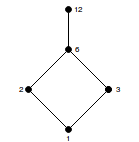
\includegraphics{ret_diagram}
\end{frame}
%------------------------------------------------

\begin{frame}
\Huge{\centerline{The End}}
\end{frame}

%----------------------------------------------------------------------------------------

\end{document} 